\documentclass[border=2pt]{standalone}
\usepackage{pgfplots}
\pgfplotsset{compat=1.18}
\begin{document}
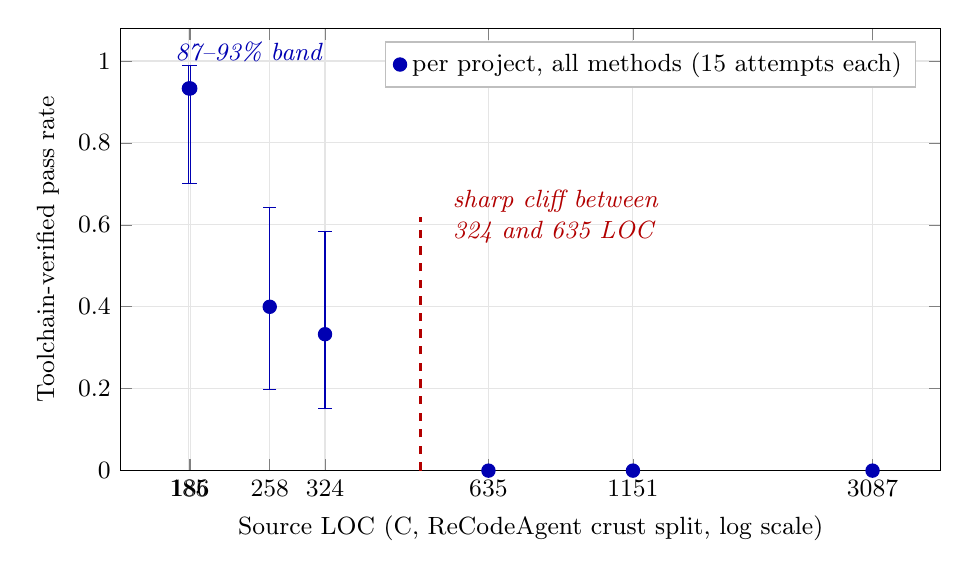
\begin{tikzpicture}
\begin{semilogxaxis}[
  width=12cm,
  height=7.2cm,
  xlabel={Source LOC (C, ReCodeAgent crust split, log scale)},
  ylabel={Toolchain-verified pass rate},
  ymin=0, ymax=1.08,
  ytick={0,0.2,0.4,0.6,0.8,1.0},
  xtick={185,186,258,324,635,1151,3087},
  xticklabels={185,186,258,324,635,1151,3087},
  grid=major,
  grid style={gray!20},
  legend style={at={(0.97,0.97)}, anchor=north east, font=\small, draw=gray!50},
  tick label style={font=\small},
  label style={font=\small},
  log ticks with fixed point,
]
% Per-project verified successes from survey 230926 (15 attempts per
% project: amp 14, ulidgen 14, chtrie 6, murmurhash_c 5, and 0 for the
% three largest). Error bars are Wilson 95% intervals (plus = hi - p,
% minus = p - lo): 14/15 -> [0.702, 0.988], 6/15 -> [0.198, 0.643],
% 5/15 -> [0.152, 0.583].
\addplot[
  only marks,
  mark=*, mark size=2.4pt,
  color=blue!70!black,
  error bars/.cd, y dir=both, y explicit,
]
table[
  x=loc, y=rate, y error plus=errplus, y error minus=errminus,
]{
loc rate errplus errminus
185 0.933 0.055 0.231
186 0.933 0.055 0.231
258 0.400 0.243 0.202
324 0.333 0.250 0.182
635 0 0 0
1151 0 0 0
3087 0 0 0
};
\addlegendentry{per project, all methods (15 attempts each)}
% Sharp capability cliff between 324 and 635 LOC.
\draw[dashed, thick, red!70!black]
  (axis cs:480,0) -- (axis cs:480,0.62)
  node[right=8pt, font=\small\itshape, text=red!70!black, align=left]
    {sharp cliff between\\324 and 635 LOC};
% 87-93% band annotation over the small two projects
\node[font=\small\itshape, text=blue!70!black, anchor=south west]
  at (axis cs:168,0.965) {87--93\% band};
\end{semilogxaxis}
\end{tikzpicture}
\end{document}
